\chapter{Problema 1}

\section{Descripción del problema}
A lo largo de un río hay n aldeas. En cada aldea, se puede alquilar una canoa para viajar a otras aldeas que estén a favor de la corriente (resulta casi imposible remar a contra corriente). Para todo posible punto de partida i y para todo posible punto de llegada j más abajo en el río (i<j), se conoce el coste de alquilar una canoa para ir desde i hasta j sea mayor que el coste total de una serie de alquileres más breves. En tal caso, se puede devolver la primera canoa (no hay costes adicionales por cambiar de canoa de esta manera).
Diseñe un algoritmo basado en programación dinámica para determinar el coste mínimo del viaje en canoa desde todos los puntos posibles de partida i a todos los posibles puntos de llegada j (i < j). Aplique dicho algoritmo en la resolución del caso cuya matriz de costos es la siguiente:
\begin{figure}
    \centering
    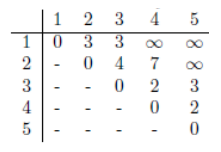
\includegraphics{figures/problema1/matriz_costes.png}
    \caption{matriz de costes}
    \label{fig:enter-label}
\end{figure}
\section{Solución: Diseño de componentes y del algoritmo}


\subsection{Resolución del problema por etapas}
En cada etapa se seleccionaría ir o no a una aldea próxima. 
Supondremos que las aldeas están ordenadas de menor a mayor coste para asegurar una solución óptima factible desde las etapas más tempranas.

\subsection{Ecuación recurrente}
Nuestra ecuación de recurrencia consta de el calculo del mínimo coste de entre  ir directamente de la aldea i hasta la aldea j  o tomar otras canoas en otras aldeas anteriores.
Siendo Coste(i,j) el coste directo de ir de i a j en canoa y MIN(i,k)+MIN(k,j)  siendo el calculo de otro camino para ir desde la aldea i hasta la aldea j alquilando otra canoa en algún pueblo anterior.
A esta ecuación de recurrencia se le añaden las restricciones de que no podemos cambiar de canoas en aldeas mas arriba del río debido a la corriente. Esto lo reflejamos con k>i y k<j. k siendo una aldea intermedia de nuestro recorrido.

\[ MIN(i, j) = min
  \left \{
    \begin{aligned}
      Coste (i, j)\\
      MIN(i, k) + MIN(k, j)    & \text{si } i<k<j
    \end{aligned}
  \right .
\]

 
\subsection{Valor objetivo}
Se desea conocer el valor OPT(i,j), el mínimo coste para realizar un viaje desde la primera aldea hasta la aldea a la que se desea llegar. 

\subsection{Verificación del cumplimiento del P.O.B}
Para demostrar que se aplica el principio de optimalidad de Bellman tenemos que demostrar que la solución óptima se consigue a partir de las soluciones óptimas los subproblemas que componen a nuestro problema. En este caso estos subproblemas son los costes mínimos de viajar desde una aldea (i) hasta otra aldea (j) para diferentes valores de i.
En este caso se cumple debido a que nuestra ecuación de recurrencia siempre va escogiendo el mínimo coste no es posible que exista una forma alternativa para ir desde la aldea i hasta la aldea j con un menor coste.

\subsection{Diseño de la memoria} 
Para el diseño de la memoria, decidimos usar una matriz en la que almacenar los costes mínimos ya calculados para ir de una aldea \textit{i} a otra \textit{j}. 
Para ello, usamos una matriz en la que se irán almacenando los valores de costes calculados. Cuando esta matriz este completa (solo la mitad superior, debido a la naturaleza del problema) se nos quedara la solución en la primera fila en forma de costes.
Cuando esto ocurra pasaremos estos costes a nuestro camino ya con el numero correspondiente a cada aldea por las que tendremos que pasar en forma de secuencia.
\subsection{Diseño del algoritmo de cálculo de coste óptimo}
\begin{lstlisting}
    calcviajeopt( matriz rio, matriz opt, salida, destino){
        para i=destino-1 hasta salida{
            para j=destino hasta i {
                opt[i][j]=rio[i][j] + min(fila j de opt)
            }
        }
        Devolver min(opt[salida])
    }
\end{lstlisting}
Para la resolución de este problema, hemos simplificado la idea de programación dinámica agregando las restricciones que nos imponía el enunciado. De esta forma, y como se puede observar en el pseudocódigo anterior, únicamente rellenaremos la mitad de la tabla(debido a la imposibilidad de acceder a una canoa que hayamos dejado atrás). Así, rellenaremos cada casilla de nuestra tabla con la distancia desde la aldea de la que procedamos hasta la que estemos comprobando en el momento, sumada a la mínima distancia posible desde esta última aldea a nuestro destino final.
Una vez la tabla se encuentre rellena, nuestra solución final corresponderá al mínimo almacenado en la fila correspondiente al punto de salida de nuestra tabla.


\subsection{Diseño del algoritmo de recuperación de la solución}
\begin{lstlisting}
    camino recuperarsol(matriz rio, matriz opt, salida, destino){
        camino = vacio
        
        minimo=min(opt[salida])
        camino += salida
        camino += minimo
        
        mientras minimo sea distinto de destino{
            minimo=min(opt[minimo])
            camino + =  minimo
        }
        Devolver camino
    }
\end{lstlisting}
Conociendo la tabla rellenada tras la ejecución del algoritmo anterior, buscaremos conocer en que aldeas hemos parado para obtener el camino a recorrer. Por ello, buscaremos el mínimo de nuestra fila de salida, añadiendo a nuestro camino tanto nuestra aldea de partida como la aldea en la que realizaremos la primera parada(correspondiente al mínimo).
A continuación realizaremos esto sucesivamente hasta llegar al destino, tomando como partida la aldea en la que hayamos realizado la parada y añadiendo a la solución únicamente las siguientes en las que vayamos a parar.
